\documentclass[1p]{elsarticle_modified}
%\bibliographystyle{elsarticle-num}

%\usepackage[colorlinks]{hyperref}
%\usepackage{abbrmath_seonhwa} %\Abb, \Ascr, \Acal ,\Abf, \Afrak
\usepackage{amsfonts}
\usepackage{amssymb}
\usepackage{amsmath}
\usepackage{amsthm}
\usepackage{scalefnt}
\usepackage{amsbsy}
\usepackage{kotex}
\usepackage{caption}
\usepackage{subfig}
\usepackage{color}
\usepackage{graphicx}
\usepackage{xcolor} %% white, black, red, green, blue, cyan, magenta, yellow
\usepackage{float}
\usepackage{setspace}
\usepackage{hyperref}

\usepackage{tikz}
\usetikzlibrary{arrows}

\usepackage{multirow}
\usepackage{array} % fixed length table
\usepackage{hhline}

%%%%%%%%%%%%%%%%%%%%%
\makeatletter
\renewcommand*\env@matrix[1][\arraystretch]{%
	\edef\arraystretch{#1}%
	\hskip -\arraycolsep
	\let\@ifnextchar\new@ifnextchar
	\array{*\c@MaxMatrixCols c}}
\makeatother %https://tex.stackexchange.com/questions/14071/how-can-i-increase-the-line-spacing-in-a-matrix
%%%%%%%%%%%%%%%

\usepackage[normalem]{ulem}

\newcommand{\msout}[1]{\ifmmode\text{\sout{\ensuremath{#1}}}\else\sout{#1}\fi}
%SOURCE: \msout is \stkout macro in https://tex.stackexchange.com/questions/20609/strikeout-in-math-mode

\newcommand{\cancel}[1]{
	\ifmmode
	{\color{red}\msout{#1}}
	\else
	{\color{red}\sout{#1}}
	\fi
}

\newcommand{\add}[1]{
	{\color{blue}\uwave{#1}}
}

\newcommand{\replace}[2]{
	\ifmmode
	{\color{red}\msout{#1}}{\color{blue}\uwave{#2}}
	\else
	{\color{red}\sout{#1}}{\color{blue}\uwave{#2}}
	\fi
}

\newcommand{\Sol}{\mathcal{S}} %segment
\newcommand{\D}{D} %diagram
\newcommand{\A}{\mathcal{A}} %arc


%%%%%%%%%%%%%%%%%%%%%%%%%%%%%5 test

\def\sl{\operatorname{\textup{SL}}(2,\Cbb)}
\def\psl{\operatorname{\textup{PSL}}(2,\Cbb)}
\def\quan{\mkern 1mu \triangleright \mkern 1mu}

\theoremstyle{definition}
\newtheorem{thm}{Theorem}[section]
\newtheorem{prop}[thm]{Proposition}
\newtheorem{lem}[thm]{Lemma}
\newtheorem{ques}[thm]{Question}
\newtheorem{cor}[thm]{Corollary}
\newtheorem{defn}[thm]{Definition}
\newtheorem{exam}[thm]{Example}
\newtheorem{rmk}[thm]{Remark}
\newtheorem{alg}[thm]{Algorithm}

\newcommand{\I}{\sqrt{-1}}
\begin{document}

%\begin{frontmatter}
%
%\title{Boundary parabolic representations of knots up to 8 crossings}
%
%%% Group authors per affiliation:
%\author{Yunhi Cho} 
%\address{Department of Mathematics, University of Seoul, Seoul, Korea}
%\ead{yhcho@uos.ac.kr}
%
%
%\author{Seonhwa Kim} %\fnref{s_kim}}
%\address{Center for Geometry and Physics, Institute for Basic Science, Pohang, 37673, Korea}
%\ead{ryeona17@ibs.re.kr}
%
%\author{Hyuk Kim}
%\address{Department of Mathematical Sciences, Seoul National University, Seoul 08826, Korea}
%\ead{hyukkim@snu.ac.kr}
%
%\author{Seokbeom Yoon}
%\address{Department of Mathematical Sciences, Seoul National University, Seoul, 08826,  Korea}
%\ead{sbyoon15@snu.ac.kr}
%
%\begin{abstract}
%We find all boundary parabolic representation of knots up to 8 crossings.
%
%\end{abstract}
%\begin{keyword}
%    \MSC[2010] 57M25 
%\end{keyword}
%
%\end{frontmatter}

%\linenumbers
%\tableofcontents
%
\newcommand\colored[1]{\textcolor{white}{\rule[-0.35ex]{0.8em}{1.4ex}}\kern-0.8em\color{red} #1}%
%\newcommand\colored[1]{\textcolor{white}{ #1}\kern-2.17ex	\textcolor{white}{ #1}\kern-1.81ex	\textcolor{white}{ #1}\kern-2.15ex\color{red}#1	}

{\Large $\underline{11a_{304}~(K11a_{304})}$}

\setlength{\tabcolsep}{10pt}
\renewcommand{\arraystretch}{1.6}
\vspace{1cm}\begin{tabular}{m{100pt}>{\centering\arraybackslash}m{274pt}}
\multirow{5}{120pt}{
	\centering
	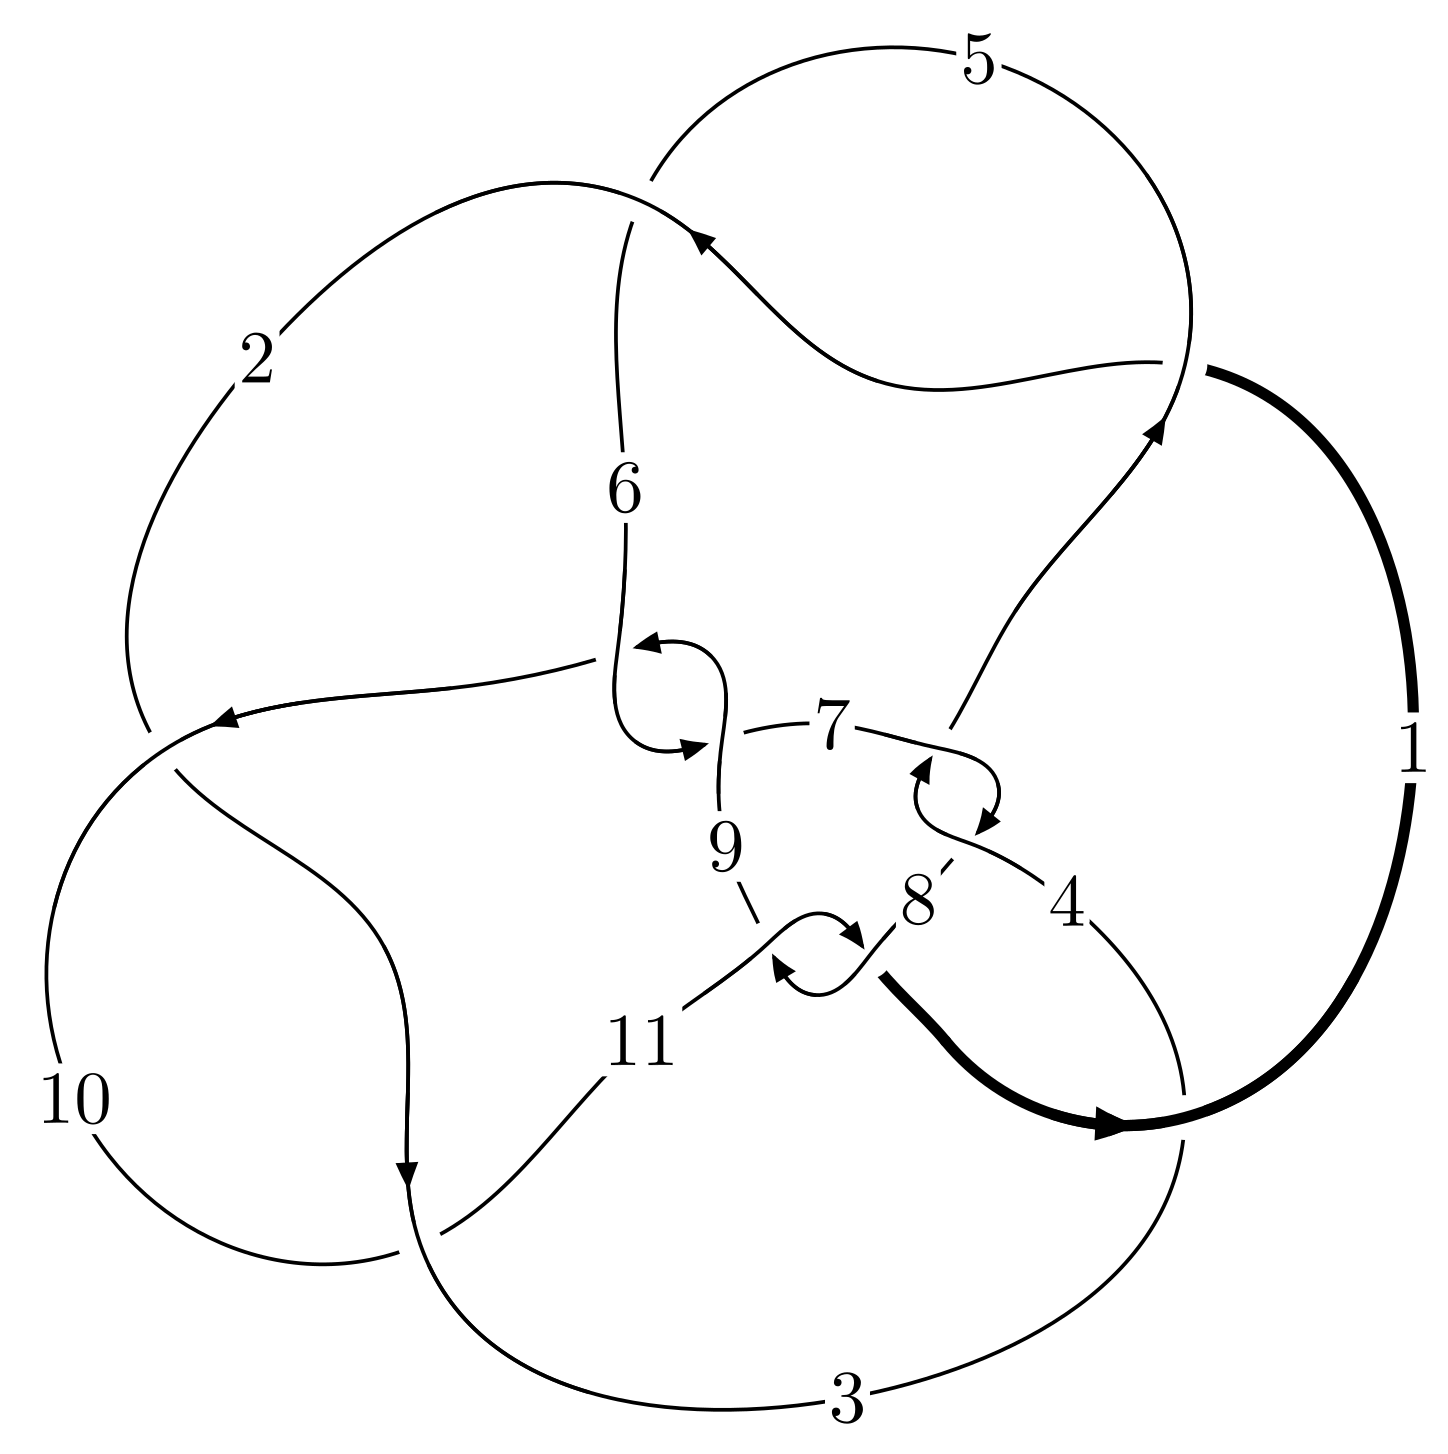
\includegraphics[width=112pt]{../../../GIT/diagram.site/Diagrams/png/553_11a_304.png}\\
\ \ \ A knot diagram\footnotemark}&
\allowdisplaybreaks
\textbf{Linearized knot diagam} \\
\cline{2-2}
 &
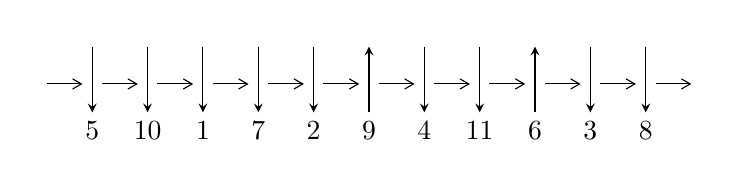
\begin{tikzpicture}[x=20pt, y=17pt]
	% nodes
	\node (C0) at (0, 0) {};
	\node (C1) at (1, 0) {};
	\node (C1U) at (1, +1) {};
	\node (C1D) at (1, -1) {5};

	\node (C2) at (2, 0) {};
	\node (C2U) at (2, +1) {};
	\node (C2D) at (2, -1) {10};

	\node (C3) at (3, 0) {};
	\node (C3U) at (3, +1) {};
	\node (C3D) at (3, -1) {1};

	\node (C4) at (4, 0) {};
	\node (C4U) at (4, +1) {};
	\node (C4D) at (4, -1) {7};

	\node (C5) at (5, 0) {};
	\node (C5U) at (5, +1) {};
	\node (C5D) at (5, -1) {2};

	\node (C6) at (6, 0) {};
	\node (C6U) at (6, +1) {};
	\node (C6D) at (6, -1) {9};

	\node (C7) at (7, 0) {};
	\node (C7U) at (7, +1) {};
	\node (C7D) at (7, -1) {4};

	\node (C8) at (8, 0) {};
	\node (C8U) at (8, +1) {};
	\node (C8D) at (8, -1) {11};

	\node (C9) at (9, 0) {};
	\node (C9U) at (9, +1) {};
	\node (C9D) at (9, -1) {6};

	\node (C10) at (10, 0) {};
	\node (C10U) at (10, +1) {};
	\node (C10D) at (10, -1) {3};

	\node (C11) at (11, 0) {};
	\node (C11U) at (11, +1) {};
	\node (C11D) at (11, -1) {8};
	\node (C12) at (12, 0) {};

	% arrows
	\draw[->,>={angle 60}]
	(C0) edge (C1) (C1) edge (C2) (C2) edge (C3) (C3) edge (C4) (C4) edge (C5) (C5) edge (C6) (C6) edge (C7) (C7) edge (C8) (C8) edge (C9) (C9) edge (C10) (C10) edge (C11) (C11) edge (C12) ;	\draw[->,>=stealth]
	(C1U) edge (C1D) (C2U) edge (C2D) (C3U) edge (C3D) (C4U) edge (C4D) (C5U) edge (C5D) (C6D) edge (C6U) (C7U) edge (C7D) (C8U) edge (C8D) (C9D) edge (C9U) (C10U) edge (C10D) (C11U) edge (C11D) ;
	\end{tikzpicture} \\
\hhline{~~} \\& 
\textbf{Solving Sequence} \\ \cline{2-2} 
 &
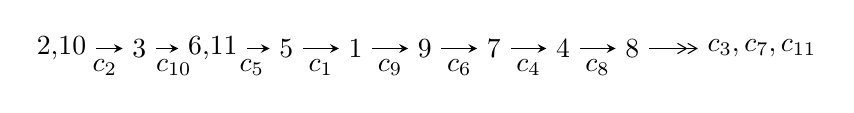
\begin{tikzpicture}[x=25pt, y=7pt]
	% node
	\node (A0) at (-1/8, 0) {2,10};
	\node (A1) at (1, 0) {3};
	\node (A2) at (33/16, 0) {6,11};
	\node (A3) at (25/8, 0) {5};
	\node (A4) at (33/8, 0) {1};
	\node (A5) at (41/8, 0) {9};
	\node (A6) at (49/8, 0) {7};
	\node (A7) at (57/8, 0) {4};
	\node (A8) at (65/8, 0) {8};
	\node (C1) at (1/2, -1) {$c_{2}$};
	\node (C2) at (3/2, -1) {$c_{10}$};
	\node (C3) at (21/8, -1) {$c_{5}$};
	\node (C4) at (29/8, -1) {$c_{1}$};
	\node (C5) at (37/8, -1) {$c_{9}$};
	\node (C6) at (45/8, -1) {$c_{6}$};
	\node (C7) at (53/8, -1) {$c_{4}$};
	\node (C8) at (61/8, -1) {$c_{8}$};
	\node (A9) at (10, 0) {$c_{3},c_{7},c_{11}$};

	% edge
	\draw[->,>=stealth]	
	(A0) edge (A1) (A1) edge (A2) (A2) edge (A3) (A3) edge (A4) (A4) edge (A5) (A5) edge (A6) (A6) edge (A7) (A7) edge (A8) ;
	\draw[->>,>={angle 60}]	
	(A8) edge (A9);
\end{tikzpicture} \\ 

\end{tabular} \\

\footnotetext{
The image of knot diagram is generated by the software ``\textbf{Draw programme}" developed by Andrew Bartholomew(\url{http://www.layer8.co.uk/maths/draw/index.htm\#Running-draw}), where we modified some parts for our purpose(\url{https://github.com/CATsTAILs/LinksPainter}).
}\phantom \\ \newline 
\centering \textbf{Ideals for irreducible components\footnotemark of $X_{\text{par}}$} 
 
\begin{align*}
I^u_{1}&=\langle 
b+u,\;-3859 u^{17}+8014 u^{16}+\cdots+13433 a-31560,\;u^{18}-9 u^{16}+\cdots+2 u-1\rangle \\
I^u_{2}&=\langle 
-6.09740\times10^{97} u^{47}+2.58938\times10^{98} u^{46}+\cdots+2.24272\times10^{98} b-1.38856\times10^{100},\\
\phantom{I^u_{2}}&\phantom{= \langle  }1.06648\times10^{100} u^{47}-4.25205\times10^{100} u^{46}+\cdots+7.15429\times10^{100} a+2.73856\times10^{102},\\
\phantom{I^u_{2}}&\phantom{= \langle  }u^{48}-3 u^{47}+\cdots+2258 u+319\rangle \\
I^u_{3}&=\langle 
b+u,\;u^7- u^6-4 u^5+3 u^4+5 u^3-4 u^2+a+1,\;u^8-4 u^6+6 u^4- u^3-3 u^2+u+1\rangle \\
\\
\end{align*}
\raggedright * 3 irreducible components of $\dim_{\mathbb{C}}=0$, with total 74 representations.\\
\footnotetext{All coefficients of polynomials are rational numbers. But the coefficients are sometimes approximated in decimal forms when there is not enough margin.}
\newpage
\renewcommand{\arraystretch}{1}
\centering \section*{I. $I^u_{1}= \langle b+u,\;-3859 u^{17}+8014 u^{16}+\cdots+13433 a-31560,\;u^{18}-9 u^{16}+\cdots+2 u-1 \rangle$}
\flushleft \textbf{(i) Arc colorings}\\
\begin{tabular}{m{7pt} m{180pt} m{7pt} m{180pt} }
\flushright $a_{2}=$&$\begin{pmatrix}1\\0\end{pmatrix}$ \\
\flushright $a_{10}=$&$\begin{pmatrix}0\\u\end{pmatrix}$ \\
\flushright $a_{3}=$&$\begin{pmatrix}1\\u^2\end{pmatrix}$ \\
\flushright $a_{6}=$&$\begin{pmatrix}0.287278 u^{17}-0.596590 u^{16}+\cdots+2.96665 u+2.34944\\- u\end{pmatrix}$ \\
\flushright $a_{11}=$&$\begin{pmatrix}- u\\- u^3+u\end{pmatrix}$ \\
\flushright $a_{5}=$&$\begin{pmatrix}0.287278 u^{17}-0.596590 u^{16}+\cdots+1.96665 u+2.34944\\- u\end{pmatrix}$ \\
\flushright $a_{1}=$&$\begin{pmatrix}-0.596590 u^{17}+0.330157 u^{16}+\cdots+1.77488 u+1.28728\\- u^2\end{pmatrix}$ \\
\flushright $a_{9}=$&$\begin{pmatrix}0.581553 u^{17}-0.0745180 u^{16}+\cdots-7.40646 u+0.419489\\0.330157 u^{17}-0.592868 u^{16}+\cdots+2.48046 u-0.596590\end{pmatrix}$ \\
\flushright $a_{7}=$&$\begin{pmatrix}-1.20948 u^{17}+0.0859823 u^{16}+\cdots+3.46899 u+0.746743\\-0.0831534 u^{17}-0.239857 u^{16}+\cdots-1.74987 u+0.522073\end{pmatrix}$ \\
\flushright $a_{4}=$&$\begin{pmatrix}-0.722102 u^{17}+0.840095 u^{16}+\cdots-0.833246 u+1.68138\\-0.833991 u^{17}+1.04913 u^{16}+\cdots-2.01772 u+0.712425\end{pmatrix}$ \\
\flushright $a_{8}=$&$\begin{pmatrix}0.661877 u^{17}+0.0748158 u^{16}+\cdots-7.07243 u+0.584828\\0.186407 u^{17}-0.456041 u^{16}+\cdots+1.92809 u-0.612596\end{pmatrix}$\\ \flushright $a_{8}=$&$\begin{pmatrix}0.661877 u^{17}+0.0748158 u^{16}+\cdots-7.07243 u+0.584828\\0.186407 u^{17}-0.456041 u^{16}+\cdots+1.92809 u-0.612596\end{pmatrix}$\\&\end{tabular}
\flushleft \textbf{(ii) Obstruction class $= -1$}\\~\\
\flushleft \textbf{(iii) Cusp Shapes $= \frac{37965}{13433} u^{17}-\frac{30147}{13433} u^{16}+\cdots-\frac{4675}{1919} u-\frac{54291}{13433}$}\\~\\
\newpage\renewcommand{\arraystretch}{1}
\flushleft \textbf{(iv) u-Polynomials at the component}\newline \\
\begin{tabular}{m{50pt}|m{274pt}}
Crossings & \hspace{64pt}u-Polynomials at each crossing \\
\hline $$\begin{aligned}c_{1},c_{2},c_{5}\\c_{10}\end{aligned}$$&$\begin{aligned}
&u^{18}-9 u^{16}+\cdots+2 u-1
\end{aligned}$\\
\hline $$\begin{aligned}c_{3}\end{aligned}$$&$\begin{aligned}
&u^{18}-17 u^{17}+\cdots+640 u-64
\end{aligned}$\\
\hline $$\begin{aligned}c_{4},c_{7},c_{8}\\c_{11}\end{aligned}$$&$\begin{aligned}
&u^{18}- u^{17}+\cdots+4 u+1
\end{aligned}$\\
\hline $$\begin{aligned}c_{6},c_{9}\end{aligned}$$&$\begin{aligned}
&u^{18}+11 u^{17}+\cdots+208 u+16
\end{aligned}$\\
\hline
\end{tabular}\\~\\
\newpage\renewcommand{\arraystretch}{1}
\flushleft \textbf{(v) Riley Polynomials at the component}\newline \\
\begin{tabular}{m{50pt}|m{274pt}}
Crossings & \hspace{64pt}Riley Polynomials at each crossing \\
\hline $$\begin{aligned}c_{1},c_{2},c_{5}\\c_{10}\end{aligned}$$&$\begin{aligned}
&y^{18}-18 y^{17}+\cdots+6 y+1
\end{aligned}$\\
\hline $$\begin{aligned}c_{3}\end{aligned}$$&$\begin{aligned}
&y^{18}-3 y^{17}+\cdots-24576 y+4096
\end{aligned}$\\
\hline $$\begin{aligned}c_{4},c_{7},c_{8}\\c_{11}\end{aligned}$$&$\begin{aligned}
&y^{18}+13 y^{17}+\cdots-14 y+1
\end{aligned}$\\
\hline $$\begin{aligned}c_{6},c_{9}\end{aligned}$$&$\begin{aligned}
&y^{18}+11 y^{17}+\cdots-12160 y+256
\end{aligned}$\\
\hline
\end{tabular}\\~\\
\newpage\flushleft \textbf{(vi) Complex Volumes and Cusp Shapes}
$$\begin{array}{c|c|c}  
\text{Solutions to }I^u_{1}& \I (\text{vol} + \sqrt{-1}CS) & \text{Cusp shape}\\
 \hline 
\begin{aligned}
u &= \phantom{-}0.408078 + 0.786624 I \\
a &= \phantom{-}0.191327 + 1.032300 I \\
b &= -0.408078 - 0.786624 I\end{aligned}
 & \phantom{-}6.34892 + 0.61291 I & -0.81864 + 1.96169 I \\ \hline\begin{aligned}
u &= \phantom{-}0.408078 - 0.786624 I \\
a &= \phantom{-}0.191327 - 1.032300 I \\
b &= -0.408078 + 0.786624 I\end{aligned}
 & \phantom{-}6.34892 - 0.61291 I & -0.81864 - 1.96169 I \\ \hline\begin{aligned}
u &= -1.181090 + 0.239212 I \\
a &= -0.11707 + 1.45553 I \\
b &= \phantom{-}1.181090 - 0.239212 I\end{aligned}
 & -5.93754 - 0.90931 I & -12.67105 + 3.59251 I \\ \hline\begin{aligned}
u &= -1.181090 - 0.239212 I \\
a &= -0.11707 - 1.45553 I \\
b &= \phantom{-}1.181090 + 0.239212 I\end{aligned}
 & -5.93754 + 0.90931 I & -12.67105 - 3.59251 I \\ \hline\begin{aligned}
u &= \phantom{-}0.108330 + 0.747006 I \\
a &= -1.32407 + 0.67886 I \\
b &= -0.108330 - 0.747006 I\end{aligned}
 & \phantom{-}5.38862 + 5.69558 I & -1.81453 - 3.55021 I \\ \hline\begin{aligned}
u &= \phantom{-}0.108330 - 0.747006 I \\
a &= -1.32407 - 0.67886 I \\
b &= -0.108330 + 0.747006 I\end{aligned}
 & \phantom{-}5.38862 - 5.69558 I & -1.81453 + 3.55021 I \\ \hline\begin{aligned}
u &= -1.275010 + 0.262336 I \\
a &= \phantom{-}1.175550 + 0.241403 I \\
b &= \phantom{-}1.275010 - 0.262336 I\end{aligned}
 & \phantom{-}0.95391 + 8.87623 I & -7.74572 - 6.85139 I \\ \hline\begin{aligned}
u &= -1.275010 - 0.262336 I \\
a &= \phantom{-}1.175550 - 0.241403 I \\
b &= \phantom{-}1.275010 + 0.262336 I\end{aligned}
 & \phantom{-}0.95391 - 8.87623 I & -7.74572 + 6.85139 I \\ \hline\begin{aligned}
u &= \phantom{-}1.33028\phantom{ +0.000000I} \\
a &= -0.683762\phantom{ +0.000000I} \\
b &= -1.33028\phantom{ +0.000000I}\end{aligned}
 & -6.40721\phantom{ +0.000000I} & -14.9220\phantom{ +0.000000I} \\ \hline\begin{aligned}
u &= \phantom{-}1.41995 + 0.20994 I \\
a &= -0.613065 + 1.144820 I \\
b &= -1.41995 - 0.20994 I\end{aligned}
 & -6.13065 - 4.90278 I & -7.01114 + 4.15155 I\\
 \hline 
 \end{array}$$\newpage$$\begin{array}{c|c|c}  
\text{Solutions to }I^u_{1}& \I (\text{vol} + \sqrt{-1}CS) & \text{Cusp shape}\\
 \hline 
\begin{aligned}
u &= \phantom{-}1.41995 - 0.20994 I \\
a &= -0.613065 - 1.144820 I \\
b &= -1.41995 + 0.20994 I\end{aligned}
 & -6.13065 + 4.90278 I & -7.01114 - 4.15155 I \\ \hline\begin{aligned}
u &= -0.542099\phantom{ +0.000000I} \\
a &= \phantom{-}0.262417\phantom{ +0.000000I} \\
b &= \phantom{-}0.542099\phantom{ +0.000000I}\end{aligned}
 & -0.811801\phantom{ +0.000000I} & -12.0990\phantom{ +0.000000I} \\ \hline\begin{aligned}
u &= \phantom{-}1.49966 + 0.40429 I \\
a &= -0.028686 + 0.907225 I \\
b &= -1.49966 - 0.40429 I\end{aligned}
 & -10.72730 - 4.74355 I & -14.8235 + 1.3888 I \\ \hline\begin{aligned}
u &= \phantom{-}1.49966 - 0.40429 I \\
a &= -0.028686 - 0.907225 I \\
b &= -1.49966 + 0.40429 I\end{aligned}
 & -10.72730 + 4.74355 I & -14.8235 - 1.3888 I \\ \hline\begin{aligned}
u &= -1.53397 + 0.54225 I \\
a &= \phantom{-}0.050667 + 1.000190 I \\
b &= \phantom{-}1.53397 - 0.54225 I\end{aligned}
 & -3.9883 + 16.2483 I & -8.61000 - 8.11381 I \\ \hline\begin{aligned}
u &= -1.53397 - 0.54225 I \\
a &= \phantom{-}0.050667 - 1.000190 I \\
b &= \phantom{-}1.53397 + 0.54225 I\end{aligned}
 & -3.9883 - 16.2483 I & -8.61000 + 8.11381 I \\ \hline\begin{aligned}
u &= \phantom{-}0.159971 + 0.264831 I \\
a &= \phantom{-}2.87602 + 0.51667 I \\
b &= -0.159971 - 0.264831 I\end{aligned}
 & -0.39235 + 1.59654 I & -2.49522 - 4.52605 I \\ \hline\begin{aligned}
u &= \phantom{-}0.159971 - 0.264831 I \\
a &= \phantom{-}2.87602 - 0.51667 I \\
b &= -0.159971 + 0.264831 I\end{aligned}
 & -0.39235 - 1.59654 I & -2.49522 + 4.52605 I\\
 \hline 
 \end{array}$$\newpage\newpage\renewcommand{\arraystretch}{1}
\centering \section*{II. $I^u_{2}= \langle -6.10\times10^{97} u^{47}+2.59\times10^{98} u^{46}+\cdots+2.24\times10^{98} b-1.39\times10^{100},\;1.07\times10^{100} u^{47}-4.25\times10^{100} u^{46}+\cdots+7.15\times10^{100} a+2.74\times10^{102},\;u^{48}-3 u^{47}+\cdots+2258 u+319 \rangle$}
\flushleft \textbf{(i) Arc colorings}\\
\begin{tabular}{m{7pt} m{180pt} m{7pt} m{180pt} }
\flushright $a_{2}=$&$\begin{pmatrix}1\\0\end{pmatrix}$ \\
\flushright $a_{10}=$&$\begin{pmatrix}0\\u\end{pmatrix}$ \\
\flushright $a_{3}=$&$\begin{pmatrix}1\\u^2\end{pmatrix}$ \\
\flushright $a_{6}=$&$\begin{pmatrix}-0.149069 u^{47}+0.594336 u^{46}+\cdots-256.237 u-38.2785\\0.271875 u^{47}-1.15457 u^{46}+\cdots+396.158 u+61.9139\end{pmatrix}$ \\
\flushright $a_{11}=$&$\begin{pmatrix}- u\\- u^3+u\end{pmatrix}$ \\
\flushright $a_{5}=$&$\begin{pmatrix}0.122806 u^{47}-0.560233 u^{46}+\cdots+139.921 u+23.6354\\0.271875 u^{47}-1.15457 u^{46}+\cdots+396.158 u+61.9139\end{pmatrix}$ \\
\flushright $a_{1}=$&$\begin{pmatrix}1.54072 u^{47}-6.38173 u^{46}+\cdots+2672.27 u+435.306\\1.99109 u^{47}-8.19373 u^{46}+\cdots+3481.47 u+562.648\end{pmatrix}$ \\
\flushright $a_{9}=$&$\begin{pmatrix}-0.0375732 u^{47}+0.143876 u^{46}+\cdots-130.196 u-23.4217\\0.460900 u^{47}-1.84389 u^{46}+\cdots+889.590 u+143.667\end{pmatrix}$ \\
\flushright $a_{7}=$&$\begin{pmatrix}-0.00542028 u^{47}+0.0383142 u^{46}+\cdots+63.9028 u+9.35070\\0.0486115 u^{47}-0.222442 u^{46}+\cdots+91.9873 u+18.1913\end{pmatrix}$ \\
\flushright $a_{4}=$&$\begin{pmatrix}0.185270 u^{47}-0.834683 u^{46}+\cdots+187.771 u+28.3446\\0.335022 u^{47}-1.41596 u^{46}+\cdots+528.630 u+82.1633\end{pmatrix}$ \\
\flushright $a_{8}=$&$\begin{pmatrix}0.456200 u^{47}-1.83795 u^{46}+\cdots+821.370 u+131.984\\0.476207 u^{47}-1.90758 u^{46}+\cdots+910.659 u+147.924\end{pmatrix}$\\ \flushright $a_{8}=$&$\begin{pmatrix}0.456200 u^{47}-1.83795 u^{46}+\cdots+821.370 u+131.984\\0.476207 u^{47}-1.90758 u^{46}+\cdots+910.659 u+147.924\end{pmatrix}$\\&\end{tabular}
\flushleft \textbf{(ii) Obstruction class $= -1$}\\~\\
\flushleft \textbf{(iii) Cusp Shapes $= 6.23467 u^{47}-25.2293 u^{46}+\cdots+11604.2 u+1881.95$}\\~\\
\newpage\renewcommand{\arraystretch}{1}
\flushleft \textbf{(iv) u-Polynomials at the component}\newline \\
\begin{tabular}{m{50pt}|m{274pt}}
Crossings & \hspace{64pt}u-Polynomials at each crossing \\
\hline $$\begin{aligned}c_{1},c_{2},c_{5}\\c_{10}\end{aligned}$$&$\begin{aligned}
&u^{48}-3 u^{47}+\cdots+2258 u+319
\end{aligned}$\\
\hline $$\begin{aligned}c_{3}\end{aligned}$$&$\begin{aligned}
&(u^{24}+4 u^{23}+\cdots+2 u+1)^{2}
\end{aligned}$\\
\hline $$\begin{aligned}c_{4},c_{7},c_{8}\\c_{11}\end{aligned}$$&$\begin{aligned}
&u^{48}-5 u^{47}+\cdots+314 u+61
\end{aligned}$\\
\hline $$\begin{aligned}c_{6},c_{9}\end{aligned}$$&$\begin{aligned}
&(u^{24}-4 u^{23}+\cdots-2 u+1)^{2}
\end{aligned}$\\
\hline
\end{tabular}\\~\\
\newpage\renewcommand{\arraystretch}{1}
\flushleft \textbf{(v) Riley Polynomials at the component}\newline \\
\begin{tabular}{m{50pt}|m{274pt}}
Crossings & \hspace{64pt}Riley Polynomials at each crossing \\
\hline $$\begin{aligned}c_{1},c_{2},c_{5}\\c_{10}\end{aligned}$$&$\begin{aligned}
&y^{48}-37 y^{47}+\cdots+318056 y+101761
\end{aligned}$\\
\hline $$\begin{aligned}c_{3}\end{aligned}$$&$\begin{aligned}
&(y^{24}+6 y^{23}+\cdots+8 y+1)^{2}
\end{aligned}$\\
\hline $$\begin{aligned}c_{4},c_{7},c_{8}\\c_{11}\end{aligned}$$&$\begin{aligned}
&y^{48}+31 y^{47}+\cdots-55164 y+3721
\end{aligned}$\\
\hline $$\begin{aligned}c_{6},c_{9}\end{aligned}$$&$\begin{aligned}
&(y^{24}+20 y^{23}+\cdots+52 y+1)^{2}
\end{aligned}$\\
\hline
\end{tabular}\\~\\
\newpage\flushleft \textbf{(vi) Complex Volumes and Cusp Shapes}
$$\begin{array}{c|c|c}  
\text{Solutions to }I^u_{2}& \I (\text{vol} + \sqrt{-1}CS) & \text{Cusp shape}\\
 \hline 
\begin{aligned}
u &= -0.507410 + 0.882826 I \\
a &= -1.098430 + 0.558103 I \\
b &= \phantom{-}1.264200 - 0.100697 I\end{aligned}
 & -4.43678 - 0.22592 I & -13.45627 + 0. I\phantom{ +0.000000I} \\ \hline\begin{aligned}
u &= -0.507410 - 0.882826 I \\
a &= -1.098430 - 0.558103 I \\
b &= \phantom{-}1.264200 + 0.100697 I\end{aligned}
 & -4.43678 + 0.22592 I & -13.45627 + 0. I\phantom{ +0.000000I} \\ \hline\begin{aligned}
u &= \phantom{-}0.762695 + 0.579511 I \\
a &= \phantom{-}0.392365 - 0.571771 I \\
b &= \phantom{-}0.154819 + 0.470368 I\end{aligned}
 & \phantom{-}1.82625 - 2.21677 I & -1.73188 + 4.68950 I \\ \hline\begin{aligned}
u &= \phantom{-}0.762695 - 0.579511 I \\
a &= \phantom{-}0.392365 + 0.571771 I \\
b &= \phantom{-}0.154819 - 0.470368 I\end{aligned}
 & \phantom{-}1.82625 + 2.21677 I & -1.73188 - 4.68950 I \\ \hline\begin{aligned}
u &= -0.737778 + 0.756607 I \\
a &= \phantom{-}0.143305 - 0.121548 I \\
b &= \phantom{-}0.916292 + 0.212779 I\end{aligned}
 & -0.282838 - 0.252163 I & -7.00000 + 0. I\phantom{ +0.000000I} \\ \hline\begin{aligned}
u &= -0.737778 - 0.756607 I \\
a &= \phantom{-}0.143305 + 0.121548 I \\
b &= \phantom{-}0.916292 - 0.212779 I\end{aligned}
 & -0.282838 + 0.252163 I & -7.00000 + 0. I\phantom{ +0.000000I} \\ \hline\begin{aligned}
u &= -0.916292 + 0.212779 I \\
a &= -0.033385 + 0.208446 I \\
b &= \phantom{-}0.737778 + 0.756607 I\end{aligned}
 & -0.282838 + 0.252163 I & -7.62766 - 0.43499 I \\ \hline\begin{aligned}
u &= -0.916292 - 0.212779 I \\
a &= -0.033385 - 0.208446 I \\
b &= \phantom{-}0.737778 - 0.756607 I\end{aligned}
 & -0.282838 - 0.252163 I & -7.62766 + 0.43499 I \\ \hline\begin{aligned}
u &= -1.084950 + 0.073103 I \\
a &= -0.008039 - 0.977174 I \\
b &= -2.83805 + 2.46715 I\end{aligned}
 & -1.83976 + 0.26235 I & \phantom{-}18.4351 + 36.8531 I \\ \hline\begin{aligned}
u &= -1.084950 - 0.073103 I \\
a &= -0.008039 + 0.977174 I \\
b &= -2.83805 - 2.46715 I\end{aligned}
 & -1.83976 - 0.26235 I & \phantom{-}18.4351 - 36.8531 I\\
 \hline 
 \end{array}$$\newpage$$\begin{array}{c|c|c}  
\text{Solutions to }I^u_{2}& \I (\text{vol} + \sqrt{-1}CS) & \text{Cusp shape}\\
 \hline 
\begin{aligned}
u &= -0.185015 + 0.891964 I \\
a &= \phantom{-}1.39762 - 0.46861 I \\
b &= -1.241010 + 0.316801 I\end{aligned}
 & -3.16425 + 4.93690 I & -9.72258 - 5.53812 I \\ \hline\begin{aligned}
u &= -0.185015 - 0.891964 I \\
a &= \phantom{-}1.39762 + 0.46861 I \\
b &= -1.241010 - 0.316801 I\end{aligned}
 & -3.16425 - 4.93690 I & -9.72258 + 5.53812 I \\ \hline\begin{aligned}
u &= -1.143710 + 0.210666 I \\
a &= -0.37949 - 1.52464 I \\
b &= -1.389740 + 0.219183 I\end{aligned}
 & -6.06530 + 3.64576 I & \phantom{-0.000000 } 0 \\ \hline\begin{aligned}
u &= -1.143710 - 0.210666 I \\
a &= -0.37949 + 1.52464 I \\
b &= -1.389740 - 0.219183 I\end{aligned}
 & -6.06530 - 3.64576 I & \phantom{-0.000000 } 0 \\ \hline\begin{aligned}
u &= \phantom{-}1.013570 + 0.603926 I \\
a &= -0.671512 + 0.079817 I \\
b &= \phantom{-}0.137025 - 0.636866 I\end{aligned}
 & \phantom{-}4.61294 - 5.64930 I & \phantom{-0.000000 } 0 \\ \hline\begin{aligned}
u &= \phantom{-}1.013570 - 0.603926 I \\
a &= -0.671512 - 0.079817 I \\
b &= \phantom{-}0.137025 + 0.636866 I\end{aligned}
 & \phantom{-}4.61294 + 5.64930 I & \phantom{-0.000000 } 0 \\ \hline\begin{aligned}
u &= \phantom{-}1.076670 + 0.546759 I \\
a &= \phantom{-}0.593477 + 0.736101 I \\
b &= \phantom{-}0.316671 - 0.434852 I\end{aligned}
 & -0.782529 + 1.065850 I & \phantom{-0.000000 } 0 \\ \hline\begin{aligned}
u &= \phantom{-}1.076670 - 0.546759 I \\
a &= \phantom{-}0.593477 - 0.736101 I \\
b &= \phantom{-}0.316671 + 0.434852 I\end{aligned}
 & -0.782529 - 1.065850 I & \phantom{-0.000000 } 0 \\ \hline\begin{aligned}
u &= -1.200180 + 0.290326 I \\
a &= -0.837459 - 0.455709 I \\
b &= -1.305520 + 0.094166 I\end{aligned}
 & -2.69997 + 4.12763 I & \phantom{-0.000000 } 0 \\ \hline\begin{aligned}
u &= -1.200180 - 0.290326 I \\
a &= -0.837459 + 0.455709 I \\
b &= -1.305520 - 0.094166 I\end{aligned}
 & -2.69997 - 4.12763 I & \phantom{-0.000000 } 0\\
 \hline 
 \end{array}$$\newpage$$\begin{array}{c|c|c}  
\text{Solutions to }I^u_{2}& \I (\text{vol} + \sqrt{-1}CS) & \text{Cusp shape}\\
 \hline 
\begin{aligned}
u &= -1.264200 + 0.100697 I \\
a &= -0.129257 + 0.980773 I \\
b &= \phantom{-}0.507410 - 0.882826 I\end{aligned}
 & -4.43678 - 0.22592 I & \phantom{-0.000000 } 0 \\ \hline\begin{aligned}
u &= -1.264200 - 0.100697 I \\
a &= -0.129257 - 0.980773 I \\
b &= \phantom{-}0.507410 + 0.882826 I\end{aligned}
 & -4.43678 + 0.22592 I & \phantom{-0.000000 } 0 \\ \hline\begin{aligned}
u &= \phantom{-}1.241010 + 0.316801 I \\
a &= -0.136900 - 1.039440 I \\
b &= \phantom{-}0.185015 + 0.891964 I\end{aligned}
 & -3.16425 - 4.93690 I & \phantom{-0.000000 } 0 \\ \hline\begin{aligned}
u &= \phantom{-}1.241010 - 0.316801 I \\
a &= -0.136900 + 1.039440 I \\
b &= \phantom{-}0.185015 - 0.891964 I\end{aligned}
 & -3.16425 + 4.93690 I & \phantom{-0.000000 } 0 \\ \hline\begin{aligned}
u &= \phantom{-}1.262020 + 0.321043 I \\
a &= -0.023468 + 0.958439 I \\
b &= -0.28931 - 1.41057 I\end{aligned}
 & \phantom{-}1.74071 - 9.53525 I & \phantom{-0.000000 } 0 \\ \hline\begin{aligned}
u &= \phantom{-}1.262020 - 0.321043 I \\
a &= -0.023468 - 0.958439 I \\
b &= -0.28931 + 1.41057 I\end{aligned}
 & \phantom{-}1.74071 + 9.53525 I & \phantom{-0.000000 } 0 \\ \hline\begin{aligned}
u &= \phantom{-}1.305520 + 0.094166 I \\
a &= \phantom{-}0.850020 - 0.294012 I \\
b &= \phantom{-}1.200180 + 0.290326 I\end{aligned}
 & -2.69997 - 4.12763 I & \phantom{-0.000000 } 0 \\ \hline\begin{aligned}
u &= \phantom{-}1.305520 - 0.094166 I \\
a &= \phantom{-}0.850020 + 0.294012 I \\
b &= \phantom{-}1.200180 - 0.290326 I\end{aligned}
 & -2.69997 + 4.12763 I & \phantom{-0.000000 } 0 \\ \hline\begin{aligned}
u &= -0.350000 + 0.566175 I \\
a &= -0.98088 + 1.39510 I \\
b &= \phantom{-}1.49434 + 0.04435 I\end{aligned}
 & -0.47769 + 2.08395 I & -4.74669 - 3.16145 I \\ \hline\begin{aligned}
u &= -0.350000 - 0.566175 I \\
a &= -0.98088 - 1.39510 I \\
b &= \phantom{-}1.49434 - 0.04435 I\end{aligned}
 & -0.47769 - 2.08395 I & -4.74669 + 3.16145 I\\
 \hline 
 \end{array}$$\newpage$$\begin{array}{c|c|c}  
\text{Solutions to }I^u_{2}& \I (\text{vol} + \sqrt{-1}CS) & \text{Cusp shape}\\
 \hline 
\begin{aligned}
u &= -0.137025 + 0.636866 I \\
a &= -0.251867 + 1.198590 I \\
b &= -1.013570 - 0.603926 I\end{aligned}
 & \phantom{-}4.61294 - 5.64930 I & -2.87192 + 2.20392 I \\ \hline\begin{aligned}
u &= -0.137025 - 0.636866 I \\
a &= -0.251867 - 1.198590 I \\
b &= -1.013570 + 0.603926 I\end{aligned}
 & \phantom{-}4.61294 + 5.64930 I & -2.87192 - 2.20392 I \\ \hline\begin{aligned}
u &= \phantom{-}1.389740 + 0.219183 I \\
a &= \phantom{-}0.345996 - 1.251770 I \\
b &= \phantom{-}1.143710 + 0.210666 I\end{aligned}
 & -6.06530 - 3.64576 I & \phantom{-0.000000 } 0 \\ \hline\begin{aligned}
u &= \phantom{-}1.389740 - 0.219183 I \\
a &= \phantom{-}0.345996 + 1.251770 I \\
b &= \phantom{-}1.143710 - 0.210666 I\end{aligned}
 & -6.06530 + 3.64576 I & \phantom{-0.000000 } 0 \\ \hline\begin{aligned}
u &= \phantom{-}0.28931 + 1.41057 I \\
a &= \phantom{-}0.770694 + 0.397207 I \\
b &= -1.262020 - 0.321043 I\end{aligned}
 & \phantom{-}1.74071 - 9.53525 I & \phantom{-0.000000 } 0 \\ \hline\begin{aligned}
u &= \phantom{-}0.28931 - 1.41057 I \\
a &= \phantom{-}0.770694 - 0.397207 I \\
b &= -1.262020 + 0.321043 I\end{aligned}
 & \phantom{-}1.74071 + 9.53525 I & \phantom{-0.000000 } 0 \\ \hline\begin{aligned}
u &= -0.316671 + 0.434852 I \\
a &= \phantom{-}1.41976 - 1.57779 I \\
b &= -1.076670 - 0.546759 I\end{aligned}
 & -0.782529 + 1.065850 I & -2.95105 - 0.35875 I \\ \hline\begin{aligned}
u &= -0.316671 - 0.434852 I \\
a &= \phantom{-}1.41976 + 1.57779 I \\
b &= -1.076670 + 0.546759 I\end{aligned}
 & -0.782529 - 1.065850 I & -2.95105 + 0.35875 I \\ \hline\begin{aligned}
u &= \phantom{-}1.40310 + 0.41281 I \\
a &= \phantom{-}0.022975 - 1.042370 I \\
b &= \phantom{-}1.58930 + 0.62087 I\end{aligned}
 & -8.17000 - 9.69978 I & \phantom{-0.000000 } 0 \\ \hline\begin{aligned}
u &= \phantom{-}1.40310 - 0.41281 I \\
a &= \phantom{-}0.022975 + 1.042370 I \\
b &= \phantom{-}1.58930 - 0.62087 I\end{aligned}
 & -8.17000 + 9.69978 I & \phantom{-0.000000 } 0\\
 \hline 
 \end{array}$$\newpage$$\begin{array}{c|c|c}  
\text{Solutions to }I^u_{2}& \I (\text{vol} + \sqrt{-1}CS) & \text{Cusp shape}\\
 \hline 
\begin{aligned}
u &= -1.49434 + 0.04435 I \\
a &= \phantom{-}0.319282 - 0.688916 I \\
b &= \phantom{-}0.350000 + 0.566175 I\end{aligned}
 & -0.47769 - 2.08395 I & \phantom{-0.000000 } 0 \\ \hline\begin{aligned}
u &= -1.49434 - 0.04435 I \\
a &= \phantom{-}0.319282 + 0.688916 I \\
b &= \phantom{-}0.350000 - 0.566175 I\end{aligned}
 & -0.47769 + 2.08395 I & \phantom{-0.000000 } 0 \\ \hline\begin{aligned}
u &= -0.154819 + 0.470368 I \\
a &= \phantom{-}0.002200 - 1.341380 I \\
b &= -0.762695 + 0.579511 I\end{aligned}
 & \phantom{-}1.82625 + 2.21677 I & -1.73188 - 4.68950 I \\ \hline\begin{aligned}
u &= -0.154819 - 0.470368 I \\
a &= \phantom{-}0.002200 + 1.341380 I \\
b &= -0.762695 - 0.579511 I\end{aligned}
 & \phantom{-}1.82625 - 2.21677 I & -1.73188 + 4.68950 I \\ \hline\begin{aligned}
u &= -1.58930 + 0.62087 I \\
a &= \phantom{-}0.057376 - 0.891861 I \\
b &= -1.40310 + 0.41281 I\end{aligned}
 & -8.17000 + 9.69978 I & \phantom{-0.000000 } 0 \\ \hline\begin{aligned}
u &= -1.58930 - 0.62087 I \\
a &= \phantom{-}0.057376 + 0.891861 I \\
b &= -1.40310 - 0.41281 I\end{aligned}
 & -8.17000 - 9.69978 I & \phantom{-0.000000 } 0 \\ \hline\begin{aligned}
u &= \phantom{-}2.83805 + 2.46715 I \\
a &= -0.168774 - 0.226636 I \\
b &= \phantom{-}1.084950 + 0.073103 I\end{aligned}
 & -1.83976 - 0.26235 I & \phantom{-0.000000 } 0 \\ \hline\begin{aligned}
u &= \phantom{-}2.83805 - 2.46715 I \\
a &= -0.168774 + 0.226636 I \\
b &= \phantom{-}1.084950 - 0.073103 I\end{aligned}
 & -1.83976 + 0.26235 I & \phantom{-0.000000 } 0\\
 \hline 
 \end{array}$$\newpage\newpage\renewcommand{\arraystretch}{1}
\centering \section*{III. $I^u_{3}= \langle b+u,\;u^7- u^6-4 u^5+3 u^4+5 u^3-4 u^2+a+1,\;u^8-4 u^6+6 u^4- u^3-3 u^2+u+1 \rangle$}
\flushleft \textbf{(i) Arc colorings}\\
\begin{tabular}{m{7pt} m{180pt} m{7pt} m{180pt} }
\flushright $a_{2}=$&$\begin{pmatrix}1\\0\end{pmatrix}$ \\
\flushright $a_{10}=$&$\begin{pmatrix}0\\u\end{pmatrix}$ \\
\flushright $a_{3}=$&$\begin{pmatrix}1\\u^2\end{pmatrix}$ \\
\flushright $a_{6}=$&$\begin{pmatrix}- u^7+u^6+4 u^5-3 u^4-5 u^3+4 u^2-1\\- u\end{pmatrix}$ \\
\flushright $a_{11}=$&$\begin{pmatrix}- u\\- u^3+u\end{pmatrix}$ \\
\flushright $a_{5}=$&$\begin{pmatrix}- u^7+u^6+4 u^5-3 u^4-5 u^3+4 u^2- u-1\\- u\end{pmatrix}$ \\
\flushright $a_{1}=$&$\begin{pmatrix}u^7-3 u^5+u^4+3 u^3-4 u^2+2\\- u^2\end{pmatrix}$ \\
\flushright $a_{9}=$&$\begin{pmatrix}- u^7+u^6+4 u^5-3 u^4-5 u^3+5 u^2+u-2\\u^6+u^5-3 u^4-2 u^3+3 u^2+u-1\end{pmatrix}$ \\
\flushright $a_{7}=$&$\begin{pmatrix}-2 u^7+7 u^5-8 u^3+3 u^2+2 u-1\\u^4+u^3- u^2- u\end{pmatrix}$ \\
\flushright $a_{4}=$&$\begin{pmatrix}u^6+u^5-2 u^4- u^3+2 u^2-2 u-1\\u^7+u^6-3 u^5-3 u^4+3 u^3+3 u^2-2 u-1\end{pmatrix}$ \\
\flushright $a_{8}=$&$\begin{pmatrix}- u^7+u^6+4 u^5-4 u^4-5 u^3+7 u^2+u-3\\u^5-2 u^3+u\end{pmatrix}$\\ \flushright $a_{8}=$&$\begin{pmatrix}- u^7+u^6+4 u^5-4 u^4-5 u^3+7 u^2+u-3\\u^5-2 u^3+u\end{pmatrix}$\\&\end{tabular}
\flushleft \textbf{(ii) Obstruction class $= 1$}\\~\\
\flushleft \textbf{(iii) Cusp Shapes $= 7 u^7+u^6-22 u^5-2 u^4+23 u^3-5 u^2- u-9$}\\~\\
\newpage\renewcommand{\arraystretch}{1}
\flushleft \textbf{(iv) u-Polynomials at the component}\newline \\
\begin{tabular}{m{50pt}|m{274pt}}
Crossings & \hspace{64pt}u-Polynomials at each crossing \\
\hline $$\begin{aligned}c_{1},c_{10}\end{aligned}$$&$\begin{aligned}
&u^8-4 u^6+6 u^4+u^3-3 u^2- u+1
\end{aligned}$\\
\hline $$\begin{aligned}c_{2},c_{5}\end{aligned}$$&$\begin{aligned}
&u^8-4 u^6+6 u^4- u^3-3 u^2+u+1
\end{aligned}$\\
\hline $$\begin{aligned}c_{3}\end{aligned}$$&$\begin{aligned}
&u^8-2 u^6- u^5+16 u^4+32 u^3+24 u^2+8 u+1
\end{aligned}$\\
\hline $$\begin{aligned}c_{4},c_{8}\end{aligned}$$&$\begin{aligned}
&u^8- u^7+4 u^6-3 u^5+6 u^4-3 u^3+3 u^2- u+1
\end{aligned}$\\
\hline $$\begin{aligned}c_{6}\end{aligned}$$&$\begin{aligned}
&u^8+2 u^7+5 u^6+2 u^5+4 u^4-2 u^3+u^2- u+1
\end{aligned}$\\
\hline $$\begin{aligned}c_{7},c_{11}\end{aligned}$$&$\begin{aligned}
&u^8+u^7+4 u^6+3 u^5+6 u^4+3 u^3+3 u^2+u+1
\end{aligned}$\\
\hline $$\begin{aligned}c_{9}\end{aligned}$$&$\begin{aligned}
&u^8-2 u^7+5 u^6-2 u^5+4 u^4+2 u^3+u^2+u+1
\end{aligned}$\\
\hline
\end{tabular}\\~\\
\newpage\renewcommand{\arraystretch}{1}
\flushleft \textbf{(v) Riley Polynomials at the component}\newline \\
\begin{tabular}{m{50pt}|m{274pt}}
Crossings & \hspace{64pt}Riley Polynomials at each crossing \\
\hline $$\begin{aligned}c_{1},c_{2},c_{5}\\c_{10}\end{aligned}$$&$\begin{aligned}
&y^8-8 y^7+28 y^6-54 y^5+62 y^4-45 y^3+23 y^2-7 y+1
\end{aligned}$\\
\hline $$\begin{aligned}c_{3}\end{aligned}$$&$\begin{aligned}
&y^8-4 y^7+36 y^6-17 y^5+226 y^4-244 y^3+96 y^2-16 y+1
\end{aligned}$\\
\hline $$\begin{aligned}c_{4},c_{7},c_{8}\\c_{11}\end{aligned}$$&$\begin{aligned}
&y^8+7 y^7+22 y^6+39 y^5+42 y^4+29 y^3+15 y^2+5 y+1
\end{aligned}$\\
\hline $$\begin{aligned}c_{6},c_{9}\end{aligned}$$&$\begin{aligned}
&y^8+6 y^7+25 y^6+46 y^5+40 y^4+18 y^3+5 y^2+y+1
\end{aligned}$\\
\hline
\end{tabular}\\~\\
\newpage\flushleft \textbf{(vi) Complex Volumes and Cusp Shapes}
$$\begin{array}{c|c|c}  
\text{Solutions to }I^u_{3}& \I (\text{vol} + \sqrt{-1}CS) & \text{Cusp shape}\\
 \hline 
\begin{aligned}
u &= \phantom{-}0.637594 + 0.491904 I \\
a &= \phantom{-}0.269821 - 0.686725 I \\
b &= -0.637594 - 0.491904 I\end{aligned}
 & \phantom{-}3.58036 - 6.89137 I & -7.40021 + 6.36507 I \\ \hline\begin{aligned}
u &= \phantom{-}0.637594 - 0.491904 I \\
a &= \phantom{-}0.269821 + 0.686725 I \\
b &= -0.637594 + 0.491904 I\end{aligned}
 & \phantom{-}3.58036 + 6.89137 I & -7.40021 - 6.36507 I \\ \hline\begin{aligned}
u &= \phantom{-}1.350130 + 0.230207 I \\
a &= -0.520365 + 1.298460 I \\
b &= -1.350130 - 0.230207 I\end{aligned}
 & -7.12528 - 4.91384 I & -15.9725 + 5.8373 I \\ \hline\begin{aligned}
u &= \phantom{-}1.350130 - 0.230207 I \\
a &= -0.520365 - 1.298460 I \\
b &= -1.350130 + 0.230207 I\end{aligned}
 & -7.12528 + 4.91384 I & -15.9725 - 5.8373 I \\ \hline\begin{aligned}
u &= -0.603955 + 0.161841 I \\
a &= \phantom{-}0.880661 - 0.975730 I \\
b &= \phantom{-}0.603955 - 0.161841 I\end{aligned}
 & -1.17049 - 1.46276 I & -13.60538 + 3.21811 I \\ \hline\begin{aligned}
u &= -0.603955 - 0.161841 I \\
a &= \phantom{-}0.880661 + 0.975730 I \\
b &= \phantom{-}0.603955 + 0.161841 I\end{aligned}
 & -1.17049 + 1.46276 I & -13.60538 - 3.21811 I \\ \hline\begin{aligned}
u &= -1.38377 + 0.43339 I \\
a &= -0.130117 + 0.725566 I \\
b &= \phantom{-}1.38377 - 0.43339 I\end{aligned}
 & -1.86433 + 0.65741 I & -7.52191 - 0.35368 I \\ \hline\begin{aligned}
u &= -1.38377 - 0.43339 I \\
a &= -0.130117 - 0.725566 I \\
b &= \phantom{-}1.38377 + 0.43339 I\end{aligned}
 & -1.86433 - 0.65741 I & -7.52191 + 0.35368 I\\
 \hline 
 \end{array}$$\newpage
\newpage\renewcommand{\arraystretch}{1}
\centering \section*{ IV. u-Polynomials}
\begin{tabular}{m{50pt}|m{274pt}}
Crossings & \hspace{64pt}u-Polynomials at each crossing \\
\hline $$\begin{aligned}c_{1},c_{10}\end{aligned}$$&$\begin{aligned}
&(u^8-4 u^6+6 u^4+u^3-3 u^2- u+1)(u^{18}-9 u^{16}+\cdots+2 u-1)\\
&\cdot(u^{48}-3 u^{47}+\cdots+2258 u+319)
\end{aligned}$\\
\hline $$\begin{aligned}c_{2},c_{5}\end{aligned}$$&$\begin{aligned}
&(u^8-4 u^6+6 u^4- u^3-3 u^2+u+1)(u^{18}-9 u^{16}+\cdots+2 u-1)\\
&\cdot(u^{48}-3 u^{47}+\cdots+2258 u+319)
\end{aligned}$\\
\hline $$\begin{aligned}c_{3}\end{aligned}$$&$\begin{aligned}
&(u^8-2 u^6- u^5+16 u^4+32 u^3+24 u^2+8 u+1)\\
&\cdot(u^{18}-17 u^{17}+\cdots+640 u-64)(u^{24}+4 u^{23}+\cdots+2 u+1)^{2}
\end{aligned}$\\
\hline $$\begin{aligned}c_{4},c_{8}\end{aligned}$$&$\begin{aligned}
&(u^8- u^7+\cdots- u+1)(u^{18}- u^{17}+\cdots+4 u+1)\\
&\cdot(u^{48}-5 u^{47}+\cdots+314 u+61)
\end{aligned}$\\
\hline $$\begin{aligned}c_{6}\end{aligned}$$&$\begin{aligned}
&(u^8+2 u^7+5 u^6+2 u^5+4 u^4-2 u^3+u^2- u+1)\\
&\cdot(u^{18}+11 u^{17}+\cdots+208 u+16)(u^{24}-4 u^{23}+\cdots-2 u+1)^{2}
\end{aligned}$\\
\hline $$\begin{aligned}c_{7},c_{11}\end{aligned}$$&$\begin{aligned}
&(u^8+u^7+\cdots+u+1)(u^{18}- u^{17}+\cdots+4 u+1)\\
&\cdot(u^{48}-5 u^{47}+\cdots+314 u+61)
\end{aligned}$\\
\hline $$\begin{aligned}c_{9}\end{aligned}$$&$\begin{aligned}
&(u^8-2 u^7+5 u^6-2 u^5+4 u^4+2 u^3+u^2+u+1)\\
&\cdot(u^{18}+11 u^{17}+\cdots+208 u+16)(u^{24}-4 u^{23}+\cdots-2 u+1)^{2}
\end{aligned}$\\
\hline
\end{tabular}\newpage\renewcommand{\arraystretch}{1}
\centering \section*{ V. Riley Polynomials}
\begin{tabular}{m{50pt}|m{274pt}}
Crossings & \hspace{64pt}Riley Polynomials at each crossing \\
\hline $$\begin{aligned}c_{1},c_{2},c_{5}\\c_{10}\end{aligned}$$&$\begin{aligned}
&(y^8-8 y^7+28 y^6-54 y^5+62 y^4-45 y^3+23 y^2-7 y+1)\\
&\cdot(y^{18}-18 y^{17}+\cdots+6 y+1)(y^{48}-37 y^{47}+\cdots+318056 y+101761)
\end{aligned}$\\
\hline $$\begin{aligned}c_{3}\end{aligned}$$&$\begin{aligned}
&(y^8-4 y^7+36 y^6-17 y^5+226 y^4-244 y^3+96 y^2-16 y+1)\\
&\cdot(y^{18}-3 y^{17}+\cdots-24576 y+4096)(y^{24}+6 y^{23}+\cdots+8 y+1)^{2}
\end{aligned}$\\
\hline $$\begin{aligned}c_{4},c_{7},c_{8}\\c_{11}\end{aligned}$$&$\begin{aligned}
&(y^8+7 y^7+22 y^6+39 y^5+42 y^4+29 y^3+15 y^2+5 y+1)\\
&\cdot(y^{18}+13 y^{17}+\cdots-14 y+1)(y^{48}+31 y^{47}+\cdots-55164 y+3721)
\end{aligned}$\\
\hline $$\begin{aligned}c_{6},c_{9}\end{aligned}$$&$\begin{aligned}
&(y^8+6 y^7+25 y^6+46 y^5+40 y^4+18 y^3+5 y^2+y+1)\\
&\cdot(y^{18}+11 y^{17}+\cdots-12160 y+256)(y^{24}+20 y^{23}+\cdots+52 y+1)^{2}
\end{aligned}$\\
\hline
\end{tabular}
\vskip 2pc
\end{document}